\section{Betrieb-, Infrastruktur- und Ausbildungskosten}
\label{s:Kosten}
In diesem Unterkapitel werden die Kostenstrukturen vorgestellt, 
wobei bei Betriebskosten auf die Kosten der Fluggesellschaft
eingegangen wird und bei der Infrastruktur, aufgrund der dazugehörigen Kapitalkosten, auf die Flughäfen.
%
\subsection{Betriebskosten einer Fluggesellschaft}

Die Betriebskosten bei einer Flugzeugabfertigung werden auf Direct Operating Costs ($DOC$), und Indirect Operating Costs 
($IOC$) geteilt, die werden auch Einzel- und Gemeinkosten genannt \cite{conrady2019luftverkehr}. 
Nach Mensen \cite{mensen2013handbuch} können $DOC$ einem bestimmten Flugzeug oder einer Strecke zugeordnet 
werden und können normalerweise als DOC pro Flugstunde, pro Kilometer, pro Passagierkilometer oder pro Blockstunde 
berechnet werden. Wobei IOC sind nicht direkt einem Flug zugewiesen, sondern für den gesamten Betrieb anfallen, wie z.B. zeitabhängige 
Instandhaltungskosten, Verwaltungskosten, Infrastrukturkosten. Nach der Beschäftigungsabhängigkeit werden die Kosten auf fixe und variable Kosten aufgeteilt. 
Fixe Kosten sind unabhängig von dem Betrieb (z.B. Kapitalkosten, Versicherung, Personalkosten), wo hingegen die variablen Kosten sich 
von der Beschäftigung ändern.
%
Die Kostenstruktur einer Fluggesellschaft kann mit der Abbildung \ref{doc} veranschaulicht werden.
%
\begin{figure}[h]
	\centering
	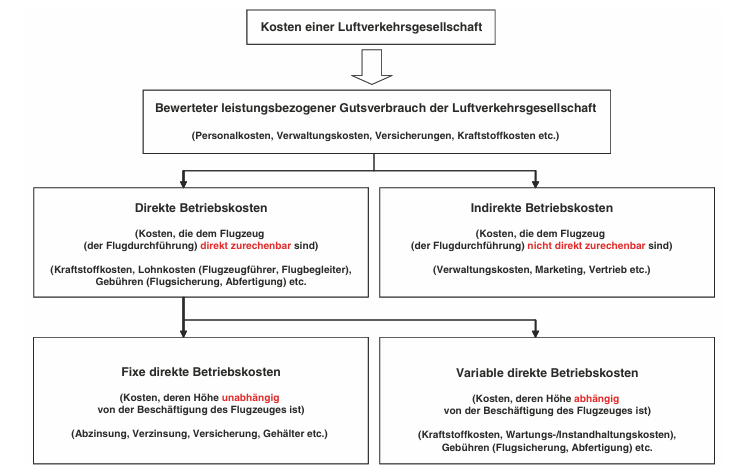
\includegraphics[width=0.9\linewidth]{Bilder/Systematik der DOC_Berechnung.png}
	\caption[Kostenstruktur einer Fluggesellschaft]{Kostenstruktur einer Fluggesellschaft \cite{mensen2013handbuch}}
	\label{doc}
\end{figure}

Betriebskosten sind von dem Flugzeugtyp abhängig, deswegen ist es wichtig vor der Anschaffung zu untersuchen, 
ob ein Flugzeug mit einem alternativen Antrieb rentabel ist. Die neuen Regularien für \ce{CO2}-Reduktion können einen Anreiz oder sogar 
eine Verpflichtung für die Fluggesellschaften schaffen, um die beste Lösung für eine Flotte zu finden. 
Mehr um politische Anreize gibt es im folgenden Unterkapitel \ref{s:Klimapolitische Maßnahmen}.
%
Es gibt verschiedene bereits vorgestellte Formeln für die Berechnung der DOC \cite{scholz_design_evaluation_doc}. 
Die meisten schließen die gleichen Kosten ein, 
unterscheiden sich jedoch mit Rechnungsweise für einzelne Kosten.\\ 
Mitberechnet werden Treibstoffkosten, Crewkosten, Wartungskosten, kapitalbezogene Kosten, sowie Entgelte und Gebühren.

%
\textbf{Treibstoffkosten} sind ein erheblicher Teil der Betriebskosten. In den USA ein Drittel von allen Gesamtkosten (TOC) aller 
Fluggesellschaften sind die Kosten für Treibstoff und Öl, vergleichsweise (in Korrelation) beträgt die Abfertigung am Flughafen ein Sechstel 
\cite{conrady2019luftverkehr}. 
Im Jahr 2023 wurden etwa 92 Milliarden Gallonen Kraftstoff durch der Luftfahrindustrie verbraucht und somit
war der Treibstoffrechnung fast 32 \% alles Betriebskosten in der Luftfahrt \cite{iata_industry_statistics_2024}.
Die jährlichen Steigerungen den Preisen für fossile Rohstoffe kann die nachhaltige Initiative fördern. \\
%Kesorinpreis im Jahr 2022 betrug USD 136/bbl, prognostiziert wird jedoch ...
%
%"Betrachtet man den aktuellen Stand der kommerziellen Luftfahrt, so macht fossiles ATF den 
%größten Teil des Energieverbrauchs im Luftverkehr aus, wobei Jet A und Jet A-1 überwiegend verwendet werden" %wo kommt das her?
%
%Technikkosten (Wartung, Reparatur, Instandhaltung MRO) - 
%es gibt unterschiedliche Typen von Wartung, die Kontrolle was am Vorfeld bei einem 
%Turnaround passiert ist die line maintenance (prüfung von Reifendruck und Ölständen), Flughafenentgelte und Handlingkosten: 
%Bodenabfertigung besteht aus Passagierabfertigung, Fracht-, Gepäckabfertigung und VorfelddiensteFlugzeugabfertigung ist direkte Kosten, 
%Passagierkosten indirekte Kosten, Kapital- und Abschreibungskosten \cite{conrady2019luftverkehr}. 
%Conrady bescheibt die Cockpit Crew als auch Cabin Crew, so Gehälter, Reisekosten, Schulungskosten. Es gibt jedoch nur wenige Arbeiten, 
%die die Ausbildungskosten erwähnen. Auch Handling Agents Kosten gibt es nicht viel Information zu finden. Es kann damit zurückgeführt werden, dass
%sind unabhängige von Fluggesellschaften Handling Agents für Abfertigung zuständig und nicht die Fluggesellschaften Kosten dafür übernehmen.
%
\textbf{Crewkosten} sind auch ein Bestandteil der direkten Betriebskosten. Zu einer Crew gehören Piloten und Kabine-Besatzung.
Nach Conrady \cite{conrady2019luftverkehr} bestehen die Besatzungskosten aus Gehälter, Reisekosten und Schulungskosten.
Es gibt jedoch nur wenige Arbeiten, die bei der Berechnung der Betriebskosten die Ausbildungskosten erwähnen. \\
%
\textbf{Wartungskosten} von einem Flugzeug fassen zusammen die Arbeitskosten für Beschäftigten und benötigten Materialien für die Wartung.
Außerdem werden die Kosten nach Wartung einer Zelle und den Triebwerken unterteilt \cite{wang2021research}. 
Meistens werden diese Komponente von unterschiedlichen Unternehmen hergestellt (Quelle).
Am Vorfeld bei der Luftfahrzeugabfertigung findet eine \textit{Line Maintenance} statt, 
dabei wird der Reifendruck und Ölstände überprüft \cite{conrady2019luftverkehr}. 
Überdies gibt es eine Reihe anderen regelmäßigen Kontrollen.
Wartungskosten sind von Auslastung eines Flugzeugs, je mehr ein Flugzeug sich im Betrieb befindet, desto größere
Wartungskosten zu erwarten. %schnellere Wartung man braucht, desto teurere Komponente man braucht.
%Wartungskosten wachsen mit der Größe des Flugzeugs, da mehr Personal oder mehr Zeit für die Wartung benötigt ist.
%
%Die Kurzstrecken-Flugzeuge sind mehr mit größerer Anzahl an Landungsgebühren und größere Treibstoffverbrauch verbunden sind, da 
%der Start und die Landung sind die Treibstoff aufwendigste Prozesse im ganzen Flug.
%
Je nach Flotte sind die Ersparnisse möglich, wenn die Fluggesellschaften mehrere Flugzeuge vom gleichen Typ anschaffen \cite{conrady2019luftverkehr}. 
In diesem Fall sind weniger Schulungen für die Techniker notwendig.\\
%
%
%Eine Reihe anderen Kosten, die für die Arbeit vielleicht nicht relevant?: Flugsicherungsgebühren, Versicherungskosten (bleiben), 
%Servicekosten, Marketing- und Vertriebskosten, Kpsten der allgemeinen Verwaltung, 
%Diese werden aufgrund der Komplexität der Berechnungen und der begrenzten Verfügbarkeit von Daten nicht weiter betrachtet.
%
%
%Preis für Treibstoffversorgung für kurzfristige Perioden kann folgend berechnet werden \cite{iata_saf_procurement_2024}: nicht sicher, ob die Formel nehme
%PRA-Bewertung (Risikobewertung??? Durchschnitt der Vorperiode) + Logistikkosten + zusätzliche Gebühren + Lieferantenmarge
%
Unter \textbf{kapitalbezogenen Kosten} sind die Kosten, die von Flugzeuganschaffungspreis abhängig. Darunter
sind die Abschreibung, Verzinsung und Versicherung zu verzeichnen.
Abschreibungskosten sind ein Teil der Kapitalkosten für das Flugzeug, die für den festgelegten Zeitraum, wo Flugzeug benutzt wird, verteilt \cite{conrady2019luftverkehr}.
Abschreibungswerte unterscheiden sich je nach Fluggesellschaft
Die Abschreibungskosten können auch auf die Infrastruktur bezogen werden. 
Flugzeuge werden gegen Rumpfschäden oder andere Arten von Schäden versichert \cite{scholz_design_evaluation_doc}  \\
%
%Conceptual_Design_and_Operating_Costs_Evaluation_of_a_19-seat_All-Electric_Aircraft_for_Regional_Aviation
%"die Zins- und Abschreibungskosten sinken tendenziell bei hoher Tagesauslastung"
%20 Prozent in Motorwartung verringert DOC um 4%
%
%
%Arten Wartung: DMC are the maintenance costs caused directly by the aircraft; 
%Wartung "line maintenance cost; periodic maintenance cost; workshop direct maintenance cost; and overhaul cost."
In dieser Arbeit wird der Fokus auf die direkten Betriebskosten gelegt und die indirekten Betriebskosten, wie Kosten für 
allgemeine Verwaltung, Marketing- und Servicekosten, werden wegen geringere Relevanz ausgelassen.\\
%
\subsection{Infrastrukturkosten}
%
Durch den Anstieg der Nachfrage oder wie in dem Fall von innovativen Antrieben sind die Änderungen an der Flughafeninfrastruktur notwendig.
Von der Infrastruktur sind abhängig welche Kapazitäten einen Flughafen hat.
Die Infrastrukturkosten eines Flughafens bestehen aus Kosten für luft- und landseitige Anlagen. Landseitige sind die Einrichtung, die zum Flughafen
gehören, wie Terminal oder administrative Gebäuden. Zur luftseitigen Infrastruktur gehören Start-/Landebahn, Rollbahn, Vorfeld, 
Flugsicherheitsinfrastruktur und -ausrüstung. Die Infrastruktur kann unterschiedlich finanziert werden.
Flughafengebühren, wie Lande-, Lärm-, Emissions-, Abstell-, Passagier- und Frachtgebühr tragen zur Finanzierung des Flughafens bei.%file:///C:/Users/henri/Desktop/Kosten/infrastrukturkosten-luftverkehr-ergebnisse-pilotrechnung_de.pdf

Infrastrukturkosten setzten sich nicht nur aus Anschaffung-/Investitionskosten (Kapitalanforderungen), sondern auch die Kosten für die Instandhaltung der Anlagen und Betriebskosten.
Kapitalkosten (wie Verzinsung und Abschreibung), die mit Infrastrukturinvestitionen zusammenhängen machen ein großer Teil an Gesamtkosten von einem Flughafen aus \cite{wittmer2011aviation}.
"Infrastrukturträger im Luftverkehr sind neben den Flughäfen die Bodenab
fertigungsdienste, Kommunikationseinrichtungen (z. B. SITA) und Flug
sicherungseinrichtungen (Radar-, Funknavigationsanlagen, Flugverkehrskontrolle 
ATC = Air traffic control)."  %file:///C:/Users/henri/Downloads/Lufrverkehr_10.1524_9783486841848.pdf
%
Flughäfen müssen wirtschaftliche Analyse nutzen, um Entscheidung über Flughafeninvestitionen zu treffen. %Bei Flughäfen mit beschränkten Bauschutzbereich muss für Erweiterung
Investitionsbeihilfen werden durch die Passagieranzahl des Flughafens bestimmt. Die Flughäfen mit mehr als fünf Millionen Passagieren
sollen ihre Kapitalkosten selbst tragen können \cite{conrady2019luftverkehr}. 
Die Flughäfen in der Deutschland sind überwiegend in der öffentlichen Hand \cite{conrady2019luftverkehr}.
%"Allein  die Planfeststellungs-  und  Genehmigungsverfahren  für große  Infrastrukturprojekte dauern in  
%Deutschland im Durchschnitt 10  bis 15 Jahre."%https://www.researchgate.net/publication/279512505_Handlungsbedarf_fur_Planung_und_Nutzung_der_Flughafeninfrastruktur_in_Deutschland_Needs_for_Action_in_Planning_and_Use_of_Airport_Infrastructure_in_Germany

Über landseitige Anlagen finanzieren sich Flughäfen über Mieten, Konzessionen und weitere Quellen. %file:///C:/Users/henri/Desktop/Kosten/infrastrukturkosten-luftverkehr-ergebnisse-pilotrechnung_de.pdf
Hat Flughafen regionale Bedeutung werden auch anderen Interessentengruppen an der Entwicklung teilnehmen.
Planung der Infrastrukturerweiterung oder -neubau muss in enger Zusammenarbeit 
zwischen Stakeholdern (Regulierungsbehörden, Mitarbeiter, Anteilseigner, Kreditoren usw) stattfinden \cite{wittmer2011aviation}.

Außerdem müssen Infrastrukturentscheidungen die Interessen der Gesellschaft treffen. %https://bmdv.bund.de/SharedDocs/DE/Anlage/G/wissenschaftlicher-beirat-gutachten-2011-1.pdf?__blob=publicationFile

Diese Arbeit wird sich auf die Anschaffungskosten für neue Infrastruktur fokussieren und nicht mit 
laufenden Kosten, wie Betriebskosten, Unterhalt- und Administrationskosten den Flughäfen, da sie untergeordnete Relevanz haben.

\subsection{Ausbildungskosten}

Die Schulungen sind ein wichtiger Teil der Ausbildung. 
%Über was geht in der annex
Nach ICAO Annex 6 muss das Schulungsprogramm eine Kompetenzschulung für alle installierten Geräte umfassen.
Aufgrund neuen erwarteten Antrieben werden neue Infrastruktur und Geräte benötigt und somit entstehen neue Notwendigkeit fürGefahren im Luftverkehr. 
%
Wegen unzureichende Datenlage in dem Bereich ist schwierig die Ausbildungsdauer und damit verbundenen Kosten präzise zu berechnen.
Aus diesem Grund wird auf eine detaillierte Analyse der Ausbildungskosten verzichtet und nur auf allgemein erforderliche Kenntnisse bei
der Schulung zusammengefasst/hinweisen. Dabei wird in dem Teil \ref{s:Neuartige Antriebe} auf die Sicherheitsaspekte und Gefahren 
beim Umgang mit jedem Antrieb eingegangen und im Teil 
\ref{s:Änderungen durch neue Antriebe, Annahmen und Methodik} Fazit für Ausbildung zusammengefasst. %unsicher
Wasserstoff: benötigt zusätzliche Fortbildung 

%Für Wasserstoff: 
%The goals of this training course include:
%• Familiarization with hydrogen safety properties.
%• To identify, evaluate, and address hydrogen system hazards.
%• To teach safe practices for design, materials selection, and hydrogen system operation.
%• physical principles and empirical observations on which these safe practices are based:
%• how to respond to emergency situations involving hydrogen
%• how to visualize safety concepts
%• identify numerous parameters important to hydrogen safety.
Die Ausbildung soll die allgemeinen Charakteristiken des Wasserstoffs, Umgang mit Wasserstoff möglich verbundene Gefahren, wie zu reagieren im Notfallsituationen
beinhalten. %(Quelle: https://www.icas.org/icas_archive/icas2024/data/papers/icas2024_1090_paper.pdf)
Die Schulungen sollten für alle Beteiligten an der Luftfahrzeugabfertigung gemacht werden.
